\chapter{二分类学习的可学习性}
\label{chap:binary-learnability}

前章的阈值0.4与0.6分对同样四封训练邮件，却在分数0.5处回答不同。新的邮件可能落在某个候选的错误区域，从而将它排除；若候选总体上经常出错，独立抽样遗漏该区域的机会随样本增加而减小。算法却会看过样本再选假设，因此我们还须排除另一种情况：许多候选中至少一个高风险假设碰巧分对全部训练邮件。样本量分析需要同时考虑单个候选的失败概率和可被选择的候选数。

我们先对有限候选求样本量，再把计数对象改为有限输入上的不同预测，以处理实数阈值等无限空间。VC维度量这种二元预测的丰富程度，一致收敛将其连接到风险保证。Rademacher与高斯复杂度进一步保留样本上的函数值，压缩与集成则利用重构或组合的机制分析输出。最后还须把统计存在落实为程序，分别核对停机和训练、预测资源。

分析始终以第~\ref{sec:learning-problem}节的二分类设定为基线：输入标签对、i.i.d.抽样、零一损失，以及第~\ref{sec:pac-learning}节的两种PAC量词。变化的是我们怎样控制候选与数据选解的复杂度。默认比较空间为$\mathcal H$；集成或可计算构造允许空间外输出时，另行注明非恰当学习。

\section{可实现的有限假设空间}
\label{sec:binary-finite-class}

先把可选阈值限为0.2、0.4、0.6、0.8。邮件分数仍可遍历$[0,1]$，只有候选假设数变成四个。这个有限空间使我们能够分别计算每个候选分对全部样本的概率，再合并这些事件。

若可实现性给出$h^\star\in\mathcal H$且总体风险为零，它在有限训练样本上也几乎必然零错误。ERM因此几乎必然可选经验风险为零者。这样的假设称为与样本\term{一致}（consistent），即分对这份样本的每个标签；它尚未被要求与总体真值处处相同。

一致假设仍可有大总体风险。错误概率20\%的候选分对一封的概率为80\%，分对$n$封独立邮件的概率为$0.8^n$。只看这批样本的ERM无法排除它。因此要保证最终选解可靠，需要限制任意高风险候选与样本一致的概率，单个候选的界还不够。

将20\%推广为容限$\varepsilon$。取$Y=\{0,1\}$和$S\sim\mathcal P^n$，先固定$h\in\mathcal H$。若$R_{\mathcal P}(h)>\varepsilon$，它分对一次观测的概率小于$1-\varepsilon$；独立抽样使全部分对的概率连乘，得到
\begin{equation}
  \mathbb P\bigl(\hat R_S(h)=0\bigr)
  =\bigl(1-R_{\mathcal P}(h)\bigr)^n
  \leq(1-\varepsilon)^n\leq e^{-n\varepsilon}.
  \label{eq:bad-consistent-hypothesis}
\end{equation}
这是固定假设的概率。ERM在抽样后才选择输出，须把其失败包含在“某个高风险假设仍与样本一致”的事件中，再对所有候选使用并集界。候选可能同时通过样本检验，并集界仍有效；有限的候选数因此转化为可计算的样本量。

\begin{theorem}[有限假设空间的可实现PAC样本量界]
\label{thm:finite-realizable-pac}
设$(X,\mathcal X)$为可测空间，$Y=\{0,1\}$取离散$\sigma$代数，
$\mathcal H\subseteq Y^X$是由可测分类器组成的非空有限集合，$\mathcal P$是
$X\times Y$上的联合分布。采用零一损失，并记
\[
 R_{\mathcal P}(h)=\mathbb P_{(x,y)\sim\mathcal P}\{h(x)\neq y\},\qquad
 \hat R_S(h)=\frac1n\sum_{i=1}^n\mathbb I\{h(x_i)\neq y_i\}.
\]
设$n\geq1$、$S=((x_i,y_i))_{i=1}^n\sim\mathcal P^n$，且存在
$h^\star\in\mathcal H$满足$R_{\mathcal P}(h^\star)=0$。对任意
$\varepsilon,\delta\in(0,1)$，若可测学习算法（允许内部随机性）以概率1输出满足
$\hat R_S(\hat h)=0$的$\hat h\in\mathcal H$，则
\begin{equation}
  \mathbb P_{S,A}\bigl(R_{\mathcal P}(\hat h)>\varepsilon\bigr)
  \leq |\mathcal H|e^{-n\varepsilon}.
  \label{eq:finite-realizable-failure}
\end{equation}
特别地，只要
\begin{equation}
  n\geq\frac{\log|\mathcal H|+\log(1/\delta)}{\varepsilon},
  \label{eq:finite-realizable-sample}
\end{equation}
算法就以至少$1-\delta$的概率输出期望风险不超过$\varepsilon$的假设；这里的概率
同时来自$S\sim\mathcal P^n$和算法的内部随机性。
\end{theorem}

\begin{proof}
可实现性使ERM几乎必然与样本一致。输出风险若超过$\varepsilon$，至少一个高风险候选通过了全部观测的检验。由此
\begin{align*}
 \mathbb P\bigl(R_{\mathcal P}(\hat h)>\varepsilon\bigr)
 &\leq \mathbb P\bigl(\exists h\in\mathcal H:
       R_{\mathcal P}(h)>\varepsilon,\ \hat R_S(h)=0\bigr)\\
 &\leq\sum_{h:R_{\mathcal P}(h)>\varepsilon}
       \mathbb P\bigl(\hat R_S(h)=0\bigr)
 \leq |\mathcal H|e^{-n\varepsilon}.
\end{align*}
将末项限制为$\delta$并解出$n$，即得式~\eqref{eq:finite-realizable-sample}。
\end{proof}

取四阈值空间且其中有零风险成员，要求成功概率至少99\%、风险至多5\%，便是$\delta=0.01$、$\varepsilon=0.05$。式~\eqref{eq:finite-realizable-sample}给出充分样本量$\lceil(\log4+\log100)/0.05\rceil=120$。任何满足可实现性的数据分布都可使用这个数，独立同分布抽取120封后，ERM达到该概率保证。上界并未声称119封或更少一定失败。

将候选从4个增至8个而固定双容限，充分上界变为$\lceil(\log8+\log100)/0.05\rceil=134$。候选翻倍只使未取整的上界增加$\log2/\varepsilon$。有限空间由此对任意容限都有分布统一的样本保证，即可实现PAC可学习。找到解需要多少计算，仍须另外核算。

上述证明利用零风险成员使ERM能选择样本一致者，再排除高风险者也一致的事件。标签有噪声时，各候选都可能出错，只能比较错误比例；高总体风险者仍可能碰巧少错。我们需要控制这种比例估计的偏差，才能判断训练比较是否延续到未来风险。

\section{不可知的有限假设空间}
\label{sec:binary-uniform-convergence}

为使数据选解的比较可靠，可以要求同一份样本准确评价全部候选。这样，即使ERM看过数据再选，经验风险也不会把高风险者误当低风险者。这种同时控制称为一致收敛。有限空间可直接逐候选求界，并支持不可知ERM；无限类则在第~\ref{sec:binary-infinite-class}节改用预测计数。

先选阈值再抽样时，所选$h$固定不变，经验风险却因样本而变。对每条观测，零一损失是均值为$R_{\mathcal P}(h)$的Bernoulli变量；$n$个损失相互独立。Hoeffding不等式因此控制经验错误比例的偏差：
\begin{equation}
 \mathbb P\left(\left|\hat R_S(h)-R_{\mathcal P}(h)\right|>\eta\right)
 \leq2e^{-2n\eta^2}.
 \label{eq:hoeffding-fixed-hypothesis}
\end{equation}
这一界尚未覆盖抽样后选择的$A(S)$。若同时检验四个阈值，ERM根据四个经验风险选择输出；只保证其中一个阈值估计准确，仍可能选中另一个偏差较大的阈值。若四者的偏差都不超过$\eta$，输出风险就至多比类内最低风险高$2\eta$：输出自身的偏差用去一个$\eta$，参照假设的偏差再用去一个$\eta$。后文将证明这两次比较。图~\ref{fig:learning-uniform-convergence}以竖线显示各自偏差；全部竖线受控时，样本选出的输出也受控。

\begin{figure}[htbp]
  \centering
  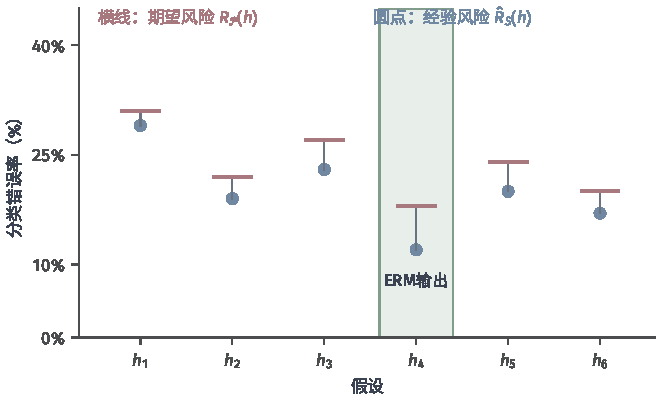
\includegraphics[width=\linewidth]{figures/03-foundations/02-learning-theory/matplotlib/learning-theory-uniform-convergence/figure.pdf}
  \caption{单个风险估计与共同保证。竖线连接各假设的经验风险与期望风险；只限制其中一条线，不能覆盖ERM在框中选择的输出。限制全部竖线后，这个数据依赖输出也落在保证内。}
  \label{fig:learning-uniform-convergence}
\end{figure}

图中的竖线表示各候选的估计偏差。固定容限$\eta$，四个阈值的风险差都不超过它，才算这份样本同时估得准。我们要找一个统一邮件数，使独立抽样得到这种共同事件的概率至少$1-\delta$，而不按未知邮件与标签分布另定样本量。下面正式定义这个要求。

\paragraph{可测性与可分性约定}

有限类的上确界是有限个可测随机变量的最大值。无限类则须处理整个零一损失函数类
\[
 \mathcal F_{01}=\{(x,y)\mapsto\ell_{01}(h(x),y):h\in\mathcal H\}
\]
本章采用第~\ref{sec:learning-problem}节给出的可测性与可分性条件，使相关上确界和比较事件可测。压缩、重构与学习器的数据依赖映射也须可测。可实现样本可选与它一致的成员，其他存在性论证采用该约定中的可测近似ERM；缺少这些条件时，以下结论不能直接沿用。

\begin{definition}[一致收敛]
\label{def:learning-uniform-convergence}
设$\mathcal H$是由可测函数$h:X\to\{0,1\}$组成的非空假设空间，采用零一损失并满足
第~\ref{sec:learning-problem}节的可测性与可分性约定。如果对
任意$\eta,\delta\in(0,1)$，都存在只依赖$\eta,\delta$和$\mathcal H$的正整数
$m_{\mathcal H}^{\mathrm{UC}}(\eta,\delta)$，使得对任意定义在$X\times\{0,1\}$上的
联合分布$\mathcal P$及任意$n\geq m_{\mathcal H}^{\mathrm{UC}}(\eta,\delta)$，独立同分布样本
$S\sim\mathcal P^n$满足
\begin{equation}
 \mathbb P_{S\sim\mathcal P^n}\left(
   \sup_{h\in\mathcal H}|\hat R_S(h)-R_{\mathcal P}(h)|\leq\eta
 \right)\geq1-\delta,
 \label{eq:learning-uniform-convergence-definition}
\end{equation}
就称$\mathcal H$满足\term{一致收敛}（uniform convergence）。
\end{definition}

式~\eqref{eq:learning-uniform-convergence-definition}的上确界覆盖$\mathcal H$中全部风险差，不必由某个假设取到。它不超过$\eta$，就表示每个候选在这份样本上估得准；对整批抽样的概率保证允许少数样本失准。$\mathcal P$是输入与标签的联合来源，包含输入频率及条件标签规律，不只是$\mathcal P_X$。各总体风险可以随分布改变，充分样本量$m_{\mathcal H}^{\mathrm{UC}}(\eta,\delta)$须保持统一。定义不要求零风险成员，故涵盖不可知设定，分布无关的范围与定义~\ref{def:general-pac-learnability}相同。

一致收敛评价的是风险估计，而非风险大小。高风险候选若在样本上也表现为高风险，仍符合估计准确的要求。

有限空间的共同偏差事件等价于没有候选的风险差超过$\eta$。式~\eqref{eq:hoeffding-fixed-hypothesis}先控制一个固定候选失准的概率，将这些有限个概率相加，就控制了至少一个候选失准的事件。

\begin{theorem}[有限假设空间的一致收敛样本量界]
\label{thm:finite-uniform-convergence}
设$(X,\mathcal X)$为可测空间，$Y=\{0,1\}$取离散$\sigma$代数，
$\mathcal H\subseteq Y^X$是由可测分类器组成的非空有限集合，$\mathcal P$是
$X\times Y$上的任意联合分布。对零一损失，记
\[
 R_{\mathcal P}(h)=\mathbb P_{(x,y)\sim\mathcal P}\{h(x)\neq y\},\qquad
 \hat R_S(h)=\frac1n\sum_{i=1}^n\mathbb I\{h(x_i)\neq y_i\}.
\]
设$n\geq1$且$S=((x_i,y_i))_{i=1}^n\sim\mathcal P^n$。对任意
$\eta,\delta\in(0,1)$，只要样本量满足
\begin{equation}
 n\geq\frac{\log(2|\mathcal H|/\delta)}{2\eta^2},
 \label{eq:finite-uniform-sample}
\end{equation}
就有
\[
 \mathbb P_{S\sim\mathcal P^n}\left(
 \sup_{h\in\mathcal H}|\hat R_S(h)-R_{\mathcal P}(h)|\leq\eta
 \right)\geq1-\delta.
\]
同一概率界也可写为：对任意$n\geq1$和$\delta\in(0,1)$，以下不等式以至少$1-\delta$的概率成立：
\begin{equation}
 \sup_{h\in\mathcal H}|\hat R_S(h)-R_{\mathcal P}(h)|
 \leq\sqrt{\frac{\log(2|\mathcal H|/\delta)}{2n}}.
 \label{eq:finite-uniform-bound}
\end{equation}
由于该样本量不依赖$\mathcal P$，有限假设空间满足分布无关的一致收敛。
\end{theorem}

\begin{proof}
对每个$h$使用式~\eqref{eq:hoeffding-fixed-hypothesis}。上确界超过$\eta$等价于至少一个候选的偏差超过$\eta$；对这些事件求并集界，得到
\[
 \mathbb P\left(\sup_{h\in\mathcal H}|\hat R_S(h)-R_{\mathcal P}(h)|>\eta\right)
 \leq 2|\mathcal H|e^{-2n\eta^2}.
\]
按式~\eqref{eq:finite-uniform-sample}选择$n$使右侧至多为$\delta$；或令右侧等于$\delta$，反解偏差$\eta$，得到式~\eqref{eq:finite-uniform-bound}。两种写法的样本要求均与具体$\mathcal P$无关。
\end{proof}

在共同准确事件上，ERM的训练比较可以变成总体比较。其输出$\hat h$的经验风险不高于任意$h\in\mathcal H$，再分别用两者的偏差界替换经验风险，即得到对总体超额风险的控制。下面据此计算有限空间的充分样本量。

\begin{theorem}[有限假设空间的不可知PAC样本量界]
\label{thm:finite-agnostic-pac}
设$(X,\mathcal X)$为可测空间，$Y=\{0,1\}$取离散$\sigma$代数，
$\mathcal H\subseteq Y^X$是由可测分类器组成的非空有限集合，$\mathcal P$是
$X\times Y$上的任意联合分布。对零一损失，记
\[
 R_{\mathcal P}(h)=\mathbb P_{(x,y)\sim\mathcal P}\{h(x)\neq y\},\qquad
 \hat R_S(h)=\frac1n\sum_{i=1}^n\mathbb I\{h(x_i)\neq y_i\}.
\]
设$n\geq1$、$S=((x_i,y_i))_{i=1}^n\sim\mathcal P^n$，可测学习算法
$A$（允许内部随机性）以概率1输出
$\hat h=A(S)\in\argmin_{h\in\mathcal H}\hat R_S(h)$。对任意
$\varepsilon,\delta\in(0,1)$，只要
\begin{equation}
 n\geq\frac{2}{\varepsilon^2}
 \left(\log(2|\mathcal H|)+\log\frac1\delta\right),
 \label{eq:finite-agnostic-sample}
\end{equation}
就有
\[
 \mathbb P_{S,A}\left(
 R_{\mathcal P}(\hat h)\leq\inf_{h\in\mathcal H}R_{\mathcal P}(h)+\varepsilon
 \right)\geq1-\delta.
\]
概率同时来自样本抽取和$A$的内部随机性。
\end{theorem}

\begin{proof}
将一致收敛容限设为$\eta=\varepsilon/2$。式~\eqref{eq:finite-agnostic-sample}使全部风险偏差不超过这个容限的概率至少为$1-\delta$。固定满足条件的样本，再取任意$h\in\mathcal H$；输出$\hat h$也在该空间内，两者均受偏差界约束。结合ERM的经验最优性，有
\begin{align*}
 R_{\mathcal P}(\hat h)
 &\leq\hat R_S(\hat h)+\frac{\varepsilon}{2}\\
 &\leq\hat R_S(h)+\frac{\varepsilon}{2}\\
 &\leq R_{\mathcal P}(h)+\varepsilon.
\end{align*}
首尾两次比较分别连接输出和参照的经验风险与总体风险，中间一次使用ERM。结论对任意$h$成立，取下确界即得所需保证。
\end{proof}

这里控制输出比类内最低风险高多少。可实现样本界的精度依赖是$1/\varepsilon$，因为只须排除高风险者全分对；不可知分析要比较可能均有错误的候选，须估准各自的错误比例。Hoeffding偏差概率按$n\eta^2$指数下降，两次偏差比较于是给出$1/\varepsilon^2$的充分界。这个差别来自评价事件的改变，不能从PAC名称推断。

同一偏差界也能落实定理~\ref{thm:srm-oracle-bound}的惩罚。设候选空间$\mathcal H_1\subseteq\mathcal H_2\subseteq\cdots$预先给定且各有限。SRM会看样本选序号$k$及$h\in\mathcal H_k$，仅保证某个预定空间准确还不够：它可能转而选中另一空间的偶然低经验风险。因此需要同时控制每个空间的全部候选。

在抽样前分配$\delta_k>0$，使$\sum_k\delta_k\leq\delta$，并对第$k$个空间设置偏差上界
\[
 p_k=\sqrt{\frac{\log(2|\mathcal H_k|/\delta_k)}{2n}}.
\]
式~\eqref{eq:finite-uniform-bound}将第$k$个空间内的失败概率控制为$\delta_k$。再跨空间使用并集界，就以至少$1-\delta$的概率在同一份样本上得到
\[
 |\hat R_S(h)-R_{\mathcal P}(h)|\leq p_k
 \qquad(k\geq1,\ h\in\mathcal H_k).
\]
这个共同事件覆盖后来选择的任意$(k,h)$，其期望风险都不超过经验风险加$p_k$。因此结构风险最小化可选择以下目标最小的组合：
\begin{equation}
 \hat R_S(h)+p_k
 \label{eq:srm-finite-penalty}
\end{equation}
扩大$\mathcal H_k$或缩小$\delta_k$都会增大惩罚。一个具体分配为$\delta_k=\delta/[k(k+1)]$；由$1/[k(k+1)]=1/k-1/(k+1)$，总预算恰为$\delta$。

失败预算还可以按空间的描述长度分配。给序号$k$预定一个二进制编码，并要求任一编码都不是另一个的开头，得到前缀编码，例如$0,10,11$标记三个空间。设编码长为$L_k$。在足够长的二进制串中，以该编码开头者占$2^{-L_k}$，不同前缀对应的串互不重叠，任意有限组的比例和便不超过1。由此全部编码也满足$\sum_k2^{-L_k}\leq1$，可以取$\delta_k=\delta2^{-L_k}$。由于$\log(1/\delta_k)=\log(1/\delta)+L_k\log2$，较长空间描述带来较小预算与较大$p_k$。这里编码只描述选哪个空间，作用是有效分配失败概率，并非PAC定义另加的必要条件。

\section{无限假设空间}
\label{sec:binary-infinite-class}

有限空间可逐候选加失败概率，无限空间这样求和则失去有限上界。我们改问：在一组有限输入上，这些函数能产生多少种不同预测？很多函数若在该组输入上回答相同，就无需在经验风险分析中分别计数。

\subsection{VC维与生长函数的学习论接口}
\label{sec:binary-shattering-vc}

\BookChapterRef{chap:combinatorics}{第一卷“数学准备”的“计数与计算”章}已建立打散、VC维、限制类$\mathcal H|_C$及\term{生长函数}（growth function）的定义。本章沿用记号
\begin{equation}
 \Pi_{\mathcal H}(m)
 =\max_{x_1,\ldots,x_m\in X}
   \left|\{(h(x_1),\ldots,h(x_m)):h\in\mathcal H\}\right|.
 \label{eq:learning-growth-function}
\end{equation}
它计算$m$个输入上最多可出现多少种二元预测。允许输入重复，因而有限输入空间也能使用任意$m$。第一卷给出阈值、单区间和平面仿射半空间的VC维$1,2,3$及前两类的精确生长函数；现在要将这些容量信息转为一致收敛和样本量保证，所需的组合上界如下。

\subsection{Sauer--Shelah引理}
\label{sec:binary-growth-sauer}

\begin{lemma}[Sauer--Shelah引理]
\label{lem:learning-sauer-shelah}
设$X$为非空集合，$\mathcal H\subseteq\{0,1\}^X$非空，并对整数$m\geq0$定义
\[
 \Pi_{\mathcal H}(m)
 =\max_{x_1,\ldots,x_m\in X}
 \left|\{(h(x_1),\ldots,h(x_m)):h\in\mathcal H\}\right|.
\]
若$1\leq d=\operatorname{VC}(\mathcal H)<\infty$，则对每个整数$m\geq d$，
\begin{equation}
 \Pi_{\mathcal H}(m)
 \leq\sum_{j=0}^{d}\binom{m}{j}
 \leq\left(\frac{em}{d}\right)^d.
 \label{eq:learning-sauer-shelah}
\end{equation}
\end{lemma}
\begin{proof}
以$G(m,d)$表示VC维至多为$d$时，$m$个输入上的最大预测数，对$m+d$强归纳。没有输入时$G(0,d)=1$；$d=0$时，每个输入的标签都唯一，故$G(m,0)=1$。

固定$m\geq1,d\geq1$及$m$个不同输入，令$V\subseteq\{0,1\}^{m}$收集预测向量。删除末坐标得到前缀集合$U$，另取能同时接上两种末标签的前缀
\[
 U'=\{u\in\{0,1\}^{m-1}:(u,0)\in V,\ (u,1)\in V\}.
\]
每个$U$中前缀贡献一次扩展，$U'$中前缀额外贡献一次，所以$|V|=|U|+|U'|$。删除坐标不会增大VC维，故$U$的VC维至多为$d$；若$U'$能打散$d$个坐标，加入末坐标后$V$就能打散$d+1$个，矛盾，故$U'$的VC维至多为$d-1$。归纳假设给出
\[
 G(m,d)\leq G(m-1,d)+G(m-1,d-1)
 \leq\sum_{j=0}^{d}\binom{m-1}{j}
   +\sum_{j=0}^{d-1}\binom{m-1}{j}.
\]
用Pascal恒等式合并两和，并约定$j>m$时$\binom mj=0$，得到$G(m,d)\leq\sum_{j=0}^{d}\binom mj$。这证明第一道不等式。

为把组合数和化为便于统计估计的表达，令$a=d/m\leq1$。在$j\leq d$时$a^j\geq a^d$，从而
\[
 a^d\sum_{j=0}^d\binom mj
 \leq\sum_{j=0}^d\binom mj a^j
 \leq(1+a)^m\leq e^{ma}=e^d.
\]
除以$a^d$即得第二道不等式。$d=0$时预测唯一，生长函数恒为1，应单独处理，避免使用以$d$作分母的公式。
\end{proof}

固定$d$时，Sauer--Shelah的界至多按$m^d$增长，全部二元预测却有$2^m$种。有限VC维因而阻止生长函数持续指数增长。它给的是上界，实际可以更慢；例如VC维3的平面仿射半空间只有$m^2$量级的预测数。

\BookChapterRef{chap:combinatorics}{第一卷“数学准备”的“计数与计算”章}用同一对数坐标对照$2^m$与有限VC维的多项式计数。差距随$m$扩大，说明可实现模式占全部组合的比例变小，候选函数本身仍可以无限。

\subsection{二分类可学习性基本定理}
\label{sec:binary-learnability-characterization}

一致收敛已说明怎样把ERM的训练比较转成总体比较。现在候选无限，所需的是所有风险差的共同概率控制。生长函数只数有限输入上的预测，接下来用第二份样本把未知总体风险换成有限输入上的可比较量。

在证明中独立抽取副样本$S'=(z_1',\ldots,z_n')$，与$S=(z_1,\ldots,z_n)$同来自联合分布$\mathcal P$，$z_i=(x_i,y_i)$。这份\term{副样本}（ghost sample）使未知风险能够通过另一份经验平均分析，学习算法不需要实际得到它。

固定$S$选定$h$后，$S'$未参与选解，因此$\hat R_{S'}(h)$对其独立评价，平均值就是$R_{\mathcal P}(h)$。若原经验风险偏离总体很大、副样本风险又接近总体，两份经验风险必有较大差异。我们因此以双样本差事件控制原样本偏差事件。此步骤只对原样本选出的那个假设使用副样本估计，尚不要求副样本同时估准全部候选。

双样本只涉及$2n$个输入，同预测的函数给出相同经验风险，故至多需要区分$\Pi_{\mathcal H}(2n)$种结果。再让每对$(z_i,z_i')$独立公平交换或保持原位。iid使联合分布不变，固定预测的差贡献则随机变号，可以应用集中不等式。将各预测的尾概率相加，就控制了任意候选产生大差的概率。副样本与随机交换构成\term{对称化}（symmetrization），作用是把总体比较转成有限计数及随机符号比较。

下面依次使用副样本、交换与预测计数，得到同时偏差的概率界。

\begin{theorem}[VC一致收敛界]
\label{thm:vc-uniform-convergence}
设$(X,\mathcal X)$为可测空间，$Y=\{0,1\}$取离散$\sigma$代数，
$\mathcal H\subseteq Y^X$是由可测分类器组成的非空集合，零一损失函数类
\[
 \mathcal F_{\mathcal H}
 =\{(x,y)\mapsto\mathbb I\{h(x)\neq y\}:h\in\mathcal H\}
\]
中的每个函数均可测，并存在可数子类$\mathcal F_0\subseteq\mathcal F_{\mathcal H}$，
使$\mathcal F_{\mathcal H}$中的每个函数都是$\mathcal F_0$中某个函数序列的逐点极限。
设$\mathcal P$是$X\times Y$上的任意联合分布，$n\geq1$，
$S=((x_i,y_i))_{i=1}^n\sim\mathcal P^n$，并记
\[
 R_{\mathcal P}(h)=\mathbb P_{(x,y)\sim\mathcal P}\{h(x)\neq y\},\qquad
 \hat R_S(h)=\frac1n\sum_{i=1}^n\mathbb I\{h(x_i)\neq y_i\},
\]
\[
 \Pi_{\mathcal H}(m)
 =\max_{x_1,\ldots,x_m\in X}
 \left|\{(h(x_1),\ldots,h(x_m)):h\in\mathcal H\}\right|.
\]
令$d=\operatorname{VC}(\mathcal H)$。对任意$\eta>0$，只要$n\eta^2\geq2$，就有
\begin{equation}
 \mathbb P_{S\sim\mathcal P^n}\left\{
   \sup_{h\in\mathcal H}|R_{\mathcal P}(h)-\hat R_S(h)|>\eta
 \right\}
 \leq4\Pi_{\mathcal H}(2n)e^{-n\eta^2/8}.
 \label{eq:vc-symmetrization-probability}
\end{equation}
因而对任意$\delta\in(0,1)$，当$1\leq d\leq2n$时，以至少$1-\delta$的概率，
\begin{equation}
 \sup_{h\in\mathcal H}|R_{\mathcal P}(h)-\hat R_S(h)|
 \leq
 \sqrt{\frac8n\left[
   d\log\frac{2en}{d}+\log\frac4\delta
 \right]}.
 \label{eq:vc-uniform-bound}
\end{equation}
若右侧大于1，则可用零一损失给出的平凡上界1替代。
\end{theorem}

\begin{proof}
引入独立副样本$S'\sim\mathcal P^n$。固定已发生原偏差事件的$S$，选$h$使$|R_{\mathcal P}(h)-\hat R_S(h)|>\eta$。条件于$S$及$h$后，副样本经验风险仍为$n$个独立Bernoulli损失的平均，故
\[
 \operatorname{Var}_{S'}\!\left(\hat R_{S'}(h)\mid S\right)
 \leq\frac{1}{4n}.
\]
用Chebyshev不等式控制它相对真实风险的偏差：
\[
 \mathbb P_{S'}\left(
   |\hat R_{S'}(h)-R_{\mathcal P}(h)|\geq\frac{\eta}{2}
   \,\middle|\,S
 \right)
 \leq\frac{1}{n\eta^2}\leq\frac12.
\]
以至少$1/2$的条件概率，副样本偏差小于$\eta/2$，这时三角不等式使两份经验风险相差大于$\eta/2$。对原样本平均后得到
\[
 \mathbb P\left\{\sup_h|R_{\mathcal P}(h)-\hat R_S(h)|>\eta\right\}
 \leq
 2\mathbb P\left\{\sup_h|\hat R_{S'}(h)-\hat R_S(h)|>\frac\eta2\right\}.
\]


固定两份样本的$2n$个观测，记配对为$(z_i,z_i')$。引入独立Rademacher符号，$\sigma_i=1$时保持该对，$\sigma_i=-1$时交换，形成$S_\sigma,S_\sigma'$。原样本独立同分布，随机交换保持联合分布；固定观测与$h$后的差值则为
\[
 \hat R_{S_\sigma'}(h)-\hat R_{S_\sigma}(h)
 =\frac1n\sum_{i=1}^n\sigma_i
 \left[\ell_{01}(h(x_i'),y_i')-\ell_{01}(h(x_i),y_i)\right].
\]
各项的取值区间长度至多$2/n$，Hoeffding给出尾界$2e^{-n\eta^2/8}$。固定输入上的预测向量至多$\Pi_{\mathcal H}(2n)$种，固定标签后每个预测向量确定一个损失向量。只对这些有限向量作并集界，得到
\[
 \mathbb P_\sigma\left\{
   \sup_h|\hat R_{S_\sigma'}(h)-\hat R_{S_\sigma}(h)|>\frac\eta2
   \,\middle|\,S,S'
 \right\}
 \leq2\Pi_{\mathcal H}(2n)e^{-n\eta^2/8}.
\]
先平均固定观测，再利用交换不改变联合分布，将这一界转回双样本差；乘上对称化的因子2，得到式~\eqref{eq:vc-symmetrization-probability}。代入Sauer--Shelah上界$\Pi_{\mathcal H}(2n)\leq(2en/d)^d$并解出失败概率$\delta$对应的偏差，即得式~\eqref{eq:vc-uniform-bound}。
\end{proof}

固定有限$d$及$\delta$，式~\eqref{eq:vc-uniform-bound}随$n$趋于零。因此任意偏差容限都能用充分样本量达到，成功概率至少$1-\delta$，且同一阈值适用于全部相关联合分布。这正是分布无关一致收敛。

一致收敛经ERM比较给不可知PAC；无限VC维则由没有免费的午餐排除可实现PAC。有限维度、两类学习与一致收敛于是形成等价关系。当前界足以建立等价性，其中对数项却未必是最优样本复杂度所必需的。

\begin{theorem}[二分类学习基本定理]
\label{thm:binary-fundamental-theorem}
设$(X,\mathcal X)$为可测空间，$Y=\{0,1\}$取离散$\sigma$代数，
$\mathcal H\subseteq Y^X$是由可测分类器组成的非空假设空间，并采用零一损失。
假定损失类
\[
 \mathcal F_{\mathcal H}
 =\{(x,y)\mapsto\mathbb I\{h(x)\neq y\}:h\in\mathcal H\}
\]
中的每个函数均可测，且存在可数子类$\mathcal F_0\subseteq\mathcal F_{\mathcal H}$，
使$\mathcal F_{\mathcal H}$中的每个函数都是$\mathcal F_0$中某个函数序列的逐点极限。
所有分布均指$X\times Y$上的联合分布，训练样本均为$S\sim\mathcal P^n$；
学习算法是可测映射并输出$\mathcal H$中的分类器，成功概率同时计入样本抽取和算法的
内部随机性。在这一分布无关设定中，下列命题等价：
\begin{enumerate}
 \item $\mathcal H$是不可知PAC可学习的；
 \item $\mathcal H$是可实现PAC可学习的；
 \item $\mathcal H$满足一致收敛；
 \item $\operatorname{VC}(\mathcal H)<\infty$。
\end{enumerate}
\end{theorem}
\begin{proof}
若VC维有限，Sauer--Shelah引理限制合并样本上的不同预测数；对称化把这种计数变成
式~\eqref{eq:vc-uniform-bound}的一致收敛界。在一致收敛事件上，ERM输出与任意比较
假设的经验风险之差不大于零，而两者的经验风险与期望风险各相差至多$\eta$，因此输出
假设的期望风险至多比$\inf_{h\in\mathcal H}R_{\mathcal P}(h)$高$2\eta$。令$\eta=\varepsilon/2$，
便得到不可知PAC可学习；不可知保证覆盖可实现分布，因而也推出可实现PAC可学习。

若VC维无限，任意$n$都能找到被打散的$2n$个输入。对任意算法，第~\ref{sec:no-free-lunch}节的定理在这些输入上给出一个可实现分布，使$n$个观测下的风险以固定正概率超过固定误差阈值。任意样本量都存在这样的分布，违反可实现PAC的统一要求，故可实现PAC可学习必有有限VC维。结合正向蕴含，四个命题等价。
\end{proof}

定理把前章的PAC量词落实为容量条件，判断是否存在统一学习保证。要使样本量与下界匹配，还须比定性可学习性更精细的分析。

\begin{theorem}[二分类的最优样本复杂度阶]
\label{thm:binary-optimal-sample-complexity}
存在普适常数$c_0\in(0,1/2)$，使以下结论成立。设$(X,\mathcal X)$为可测空间，
$Y=\{0,1\}$取离散$\sigma$代数，$\mathcal H\subseteq Y^X$是由可测分类器组成的
非空假设空间，$2\leq d=\operatorname{VC}(\mathcal H)<\infty$。假定零一损失类中的
函数均可测，并存在可数损失子类，使每个损失函数都是该子类中某个函数序列的逐点极限。
对所有$\varepsilon,\delta\in(0,c_0]$，令训练样本$S\sim\mathcal P^n$，其中
$\mathcal P$遍历$X\times Y$上的联合分布，成功概率同时计入样本抽取和学习算法的
内部随机性。在允许算法输出任意可测二分类器的分布无关极小极大意义下，可实现PAC学习的
最优样本复杂度阶为
\[
 \Theta\left(\frac{d+\log(1/\delta)}{\varepsilon}\right),
\]
不可知PAC学习的最优样本复杂度阶为
\[
 \Theta\left(\frac{d+\log(1/\delta)}{\varepsilon^2}\right).
\]
这里的$\Theta$上下界常数均为与$\mathcal H,\varepsilon,\delta$无关的普适常数。
\end{theorem}

匹配的最优阶需要上下界，不能单靠定理~\ref{thm:vc-uniform-convergence}获得。经典可实现ERM分析有额外$\log(1/\varepsilon)$，精细的非恰当学习器可去掉它\scite{hanneke2016optimal,shalevshwartz2014}。任意ERM或恰当输出不因此都达到相同阶，$d=0,1$也须另处理。统计最优仍未给出易算程序，计算条件留待章末。

\section{估计期望风险}
\label{sec:rademacher-complexity}

VC维回答了二分类是否能统一学习。对于样本已经选出的一个假设，我们还想知道它的总体风险上限。经验损失可直接计算，未知来源上的损失则需要在经验值之外补一个偏差控制量。

VC界按全输入空间的打散能力控制偏差，尚未利用当前样本位置和函数值。Rademacher与高斯复杂度保留这些信息，给出“经验风险加复杂度及抽样误差”的高概率上界。这里估计的是风险上限，没有宣称有限样本能够精确恢复未知总体风险。

\subsection{Rademacher复杂度}

\BookSectionRef{sec:probability-uniform-errors-symmetry}{第一卷“随机变量”章的“对称化与随机复杂度”一节}已定义随机复杂度并计算线性类。本章首先控制经验均值低估期望的方向，故使用不带绝对值的单侧版本。对$S=(z_1,\ldots,z_n)$与非空实值类$\mathcal G$，定义
\begin{equation}
 \widehat{\mathfrak R}_S(\mathcal G)
 =\mathbb E_\sigma\left[\sup_{f\in\mathcal G}
       \frac1n\sum_{i=1}^n\sigma_i f(z_i)\right].
 \label{eq:learning-empirical-rademacher}
\end{equation}
符号$\sigma_i$独立且等概率取$-1,1$，再对样本平均得到
\[
 \mathfrak R_n(\mathcal G)=\mathbb E_{S\sim\mathcal P^n}
       \widehat{\mathfrak R}_S(\mathcal G).
\]
第一卷的带绝对值版本在取负封闭的类上与此相同，一般则不小于当前版本。使用收缩或比较结果时须按版本核对常数。

\subsection{线性预测的复杂度}

对线性得分$f_{\bm w}(\bm x)=\bm w^\top\bm x$，随机相关和可写成$\bm w^\top\sum_i\sigma_i\bm x_i$。若参数不受限且后一个向量非零，这个量可任意增大，复杂度便不能给出有限控制。为此设$B>0$并限制$\|\bm w\|_2\leq B$，取$\mathcal F=\{\bm x\mapsto\bm w^\top\bm x:\|\bm w\|_2\leq B\}$，假定每个样本输入满足$\|\bm x_i\|_2\leq r$。以$S_X=(\bm x_1,\ldots,\bm x_n)$记输入样本，先计算得分复杂度：
\begin{align}
 \widehat{\mathfrak R}_{S_X}(\mathcal F)
 &=\frac1n\mathbb E_\sigma\sup_{\lVert\bm{w}\rVert_2\leq B}
   \bm{w}^\top\sum_i\sigma_i \bm{x}_i\nonumber\\
 &\leq\frac{B}{n}\sqrt{\sum_i\lVert\bm{x}_i\rVert_2^2}
 \leq\frac{Br}{\sqrt n}.
 \label{eq:linear-rademacher-bound}
\end{align}
固定符号时，参数沿$\sum_i\sigma_i\bm x_i$方向取长度$B$即可达到最大内积。用均方范数的平方根上界期望范数，独立符号又使交叉项的期望为零，剩下$\sum_i\|\bm x_i\|_2^2$。上界虽未显式含维数，却依赖$B$和$r$受控；缺少半径约束时，不能宣称维数无关。

\subsection{由Rademacher复杂度估计期望风险}

预测得分的复杂度还须转为损失的复杂度，才能评价风险。设$\ell\in[0,1]$，对$z=(x,y)$定义$g_h(z)=\ell(h(x),y)$，组成$\mathcal G=\{g_h:h\in\mathcal H\}$。样本均值为$\hat R_S(h)$，总体均值为$R_{\mathcal P}(h)$；控制两者之差，就能由训练值上界总体风险。

\begin{theorem}[Rademacher复杂度给出的期望风险上界]
\label{thm:rademacher-risk-bound}
设$(Z,\mathcal A)$为可测空间，$\mathcal P$为$Z$上的概率分布，$n\geq1$，
$S=(z_1,\ldots,z_n)\sim\mathcal P^n$。令$\mathcal G$为抽样前确定的、从$Z$到
$[0,1]$的非空可测函数空间；假定存在可数子类$\mathcal G_0\subseteq\mathcal G$，
使$\mathcal G$中的每个函数都是$\mathcal G_0$中某个函数序列的逐点极限。对独立于
$S$且相互独立、等概率取$-1,1$的随机变量$\sigma_1,\ldots,\sigma_n$，定义
\[
 \widehat{\mathfrak R}_S(\mathcal G)
 =\mathbb E_\sigma\left[\sup_{g\in\mathcal G}
   \frac1n\sum_{i=1}^n\sigma_i g(z_i)\right],\qquad
 \mathfrak R_n(\mathcal G)
 =\mathbb E_{S\sim\mathcal P^n}\widehat{\mathfrak R}_S(\mathcal G).
\]
则对任意$\delta\in(0,1)$，以关于$S\sim\mathcal P^n$至少$1-\delta$的概率，
对所有$g\in\mathcal G$同时有
\begin{equation}
 \mathbb E_{z\sim\mathcal P}g(z)
 \leq\frac1n\sum_i g(z_i)+2\mathfrak R_n(\mathcal G)
 +\sqrt{\frac{\log(1/\delta)}{2n}}.
 \label{eq:rademacher-risk-bound}
\end{equation}
另有一个由样本确定的上界：以关于$S\sim\mathcal P^n$至少$1-\delta$的概率，
对所有$g\in\mathcal G$同时有
\begin{equation}
 \mathbb E_{z\sim\mathcal P}g(z)
 \leq\frac1n\sum_i g(z_i)+2\widehat{\mathfrak R}_S(\mathcal G)
 +3\sqrt{\frac{\log(2/\delta)}{2n}}.
 \label{eq:empirical-rademacher-risk-bound}
\end{equation}
\end{theorem}

\begin{proof}
令$\Phi(S)=\sup_{g\in\mathcal G}(\mathbb E g-n^{-1}\sum_i g(z_i))$，即经验均值在整个类上的最大低估。引入独立副样本，用“先选择函数再平均”上界“先平均再选择”，得
\[
 \mathbb E_S\Phi(S)
 \leq\mathbb E_{S,S'}\sup_{g\in\mathcal G}
 \frac1n\sum_i\bigl(g(z_i')-g(z_i)\bigr).
\]
对每对观测随机交换，将独立符号$\sigma_i$引入差值而不改变期望。把两样本和各自取上确界，再用$\sigma_i$与$-\sigma_i$同分布，得到
\begin{equation}
 \mathbb E_S\Phi(S)\leq2\mathfrak R_n(\mathcal G).
 \label{eq:rademacher-symmetrization}
\end{equation}


替换一个观测使$\Phi(S)$最多变化$1/n$。有界差分不等式使它以至少$1-\delta$的概率不超过期望加$\sqrt{\log(1/\delta)/(2n)}$，结合上式证明第一界。经验Rademacher复杂度替换一个观测也至多变化$1/n$，所以以至少$1-\delta/2$的概率，
\[
 \mathfrak R_n(\mathcal G)
 \leq\widehat{\mathfrak R}_S(\mathcal G)
 +\sqrt{\frac{\log(2/\delta)}{2n}}.
\]
再把第一界的失败预算设为$\delta/2$，两个事件的共同概率至少$1-\delta$。替换其中的期望复杂度并合并三项偏差，得到第二界。
\end{proof}

取$g=g_h$后，定理分别给出总体风险与经验风险，另外两项是替换平均所需的复杂度及抽样代价。共同保证覆盖全部$h$，所以也覆盖数据选解。经验版本可按当前样本估复杂度，同VC维空间也可能因样本函数值不同得到不同风险界，这正是数据相关分析的用途\scite{bartlettmendelson2002}。

得分与零一损失不是同一个函数。若损失对得分为$L$-Lipschitz，改变$a$的得分至多改变$L|a|$损失，\term{收缩引理}（contraction lemma）便能将预测复杂度转成损失复杂度。其单侧和绝对值版本见\BookSectionRef{sec:probability-uniform-errors-symmetry}{第一卷“随机变量”章的“候选族的共同误差”一节}。本章用单侧版本；$\phi(0)\neq0$时先减该常数，随机和的期望不变。只有核对这种变化率条件之后才能转界，式~\eqref{eq:linear-rademacher-bound}本身不是零一风险界。

将得分复杂度转为分类风险，还要选择损失。取$y\in\{-1,1\}$、$f(\bm x)=\bm w^\top\bm x$，则$yf(\bm x)$为带符号的分类间隔：正值表示方向正确，绝对大小在得分尺度上衡量距阈值0的距离。几何间隔还须除以$\|\bm w\|_2$。对固定$\rho>0$，用下列间隔损失同时惩罚错分和不足的正间隔：
\[
 \ell_\rho(f(\bm x),y)=
 \begin{cases}
  1,&yf(\bm x)\leq0,\\
  1-yf(\bm x)/\rho,&0<yf(\bm x)<\rho,\\
  0,&yf(\bm x)\geq\rho.
 \end{cases}
\]
它在错分时为1，在正确但间隔小于$\rho$时仍为正，取值于$[0,1]$、关于得分为$1/\rho$-Lipschitz，且支配零一损失。若$\|\bm w\|_2\leq B$、$\|\bm x\|_2\leq r$几乎处处成立，收缩引理将式~\eqref{eq:linear-rademacher-bound}转为损失复杂度$Br/(\rho\sqrt n)$。风险上界因而以至少$1-\delta$的概率同时覆盖所有这些线性得分：
\begin{equation}
 R_{\mathcal P}^{01}(\operatorname{sign}f)
 \leq\frac1n\sum_i\ell_\rho(f(\bm x_i),y_i)
 +\frac{2Br}{\rho\sqrt n}
 +\sqrt{\frac{\log(1/\delta)}{2n}}.
 \label{eq:rademacher-margin-risk}
\end{equation}
这里$R_{\mathcal P}^{01}$采用零一损失，得分为0时的分类规则预先固定。若经验间隔损失为零，使右侧至多为$\varepsilon$的一项充分样本量为$O(((Br/\rho)^2+\log(1/\delta))/\varepsilon^2)$。控制量是范数与间隔的比值；高维而间隔较大时，它可能优于仅依据半空间VC维的保证。

范数、输入界和小间隔损失是这条保证额外利用的条件，并未改变二分类基本定理。只缩放参数而不改分类符号，间隔通常也缩小，风险界不能据此保证改善。数据相关复杂度可利用具体值并推广实值损失，却未承诺总比VC样本界小，也未使无限VC二类空间在全部分布上可学习。

ERM还要比较输出与参照的两个风险，故需双侧偏差。将第一界分别应用于$\mathcal G$和$1-\mathcal G=\{1-g:g\in\mathcal G\}$，两者均取值于$[0,1]$。平移不改变总体与经验均值之差，符号对称性又给出$\mathfrak R_n(1-\mathcal G)=\mathfrak R_n(\mathcal G)$。各分配$\delta/2$后，以至少$1-\delta$的概率有
\[
 |R_{\mathcal P}(h)-\hat R_S(h)|
 \leq2\mathfrak R_n(\mathcal G)+\sqrt{\frac{\log(2/\delta)}{2n}}.
\]
沿用两次偏差比较，ERM的超额风险因此满足
\begin{equation}
 R_{\mathcal P}(\hat h)-\inf_{h\in\mathcal H}R_{\mathcal P}(h)
 \leq4\mathfrak R_n(\mathcal G)
 +2\sqrt{\frac{\log(2/\delta)}{2n}}.
 \label{eq:rademacher-excess-risk}
\end{equation}
对固定分布，$\mathfrak R_n(\mathcal G)\to0$使输出风险以高概率趋近类内下确界。若有对全部允许分布成立的统一上界$\mathfrak R_n(\mathcal G)\leq a_n\to0$，才可从中选择分布无关的样本量，得到不可知PAC。单个分布上的小复杂度不等于这一统一保证。

\subsection{高斯复杂度}

\BookSectionRef{sec:probability-uniform-errors-symmetry}{第一卷“随机变量”章的“对称化与随机复杂度”一节}还给出高斯复杂度及比较关系。对独立标准高斯系数$\xi_i$，本章取单侧\term{经验高斯复杂度}（empirical Gaussian complexity）
\[
 \widehat{\mathfrak G}_S(\mathcal G)
 =\mathbb E_\xi\left[\sup_{g\in\mathcal G}\frac1n\sum_i \xi_i g(z_i)\right].
\]
高斯幅度可变，而Rademacher幅度恒为1，二者一般不能双向由普适常数比较。将$\xi_i$写成$\sigma_i|\xi_i|$，由上确界的凸性得到$\widehat{\mathfrak G}_S(\mathcal G)\geq\sqrt{2/\pi}\,\widehat{\mathfrak R}_S(\mathcal G)$。若已有高斯上界$b(S)$，便得Rademacher上界$\sqrt{\pi/2}\,b(S)$，可代入式~\eqref{eq:empirical-rademacher-risk-bound}。

将这种比较代入经验风险式，就得到以高斯复杂度表示的总体风险上界。

\begin{theorem}[高斯复杂度给出的期望风险上界]
\label{thm:gaussian-risk-bound}
设$(Z,\mathcal A)$为可测空间，$\mathcal P$为$Z$上的概率分布，$n\geq1$，
$S=(z_1,\ldots,z_n)\sim\mathcal P^n$。令
$\mathcal G=\{g_h:h\in\mathcal H\}$为抽样前确定的、从$Z$到$[0,1]$的非空可测
损失函数空间，并存在可数子类$\mathcal G_0\subseteq\mathcal G$，使$\mathcal G$
中的每个函数都是$\mathcal G_0$中某个函数序列的逐点极限。定义
\[
 R_{\mathcal P}(h)=\mathbb E_{z\sim\mathcal P}g_h(z),\qquad
 \hat R_S(h)=\frac1n\sum_{i=1}^n g_h(z_i),
\]
并对独立于$S$的独立标准高斯变量$\xi_1,\ldots,\xi_n$定义
\[
 \widehat{\mathfrak G}_S(\mathcal G)
 =\mathbb E_\xi\left[\sup_{g\in\mathcal G}
   \frac1n\sum_{i=1}^n\xi_i g(z_i)\right].
\]
则对任意$\delta\in(0,1)$，以关于$S\sim\mathcal P^n$至少$1-\delta$的概率，
所有$h\in\mathcal H$同时满足
\begin{equation}
 R_{\mathcal P}(h)\leq\hat R_S(h)
 +\sqrt{2\pi}\,\widehat{\mathfrak G}_S(\mathcal G)
 +3\sqrt{\frac{\log(2/\delta)}{2n}}.
 \label{eq:gaussian-risk-bound}
\end{equation}
\end{theorem}

\begin{proof}
将$g=g_h$代入式~\eqref{eq:empirical-rademacher-risk-bound}，再用$2\widehat{\mathfrak R}_S(\mathcal G)\leq\sqrt{2\pi}\,\widehat{\mathfrak G}_S(\mathcal G)$替换复杂度项，即得结论。
\end{proof}

使用时计算输出的经验风险，再为损失类的经验高斯复杂度求上界，代入式~\eqref{eq:gaussian-risk-bound}。已知$b(S)$时可直接替换复杂度项。由于事件同时覆盖全部候选，输出即使在看过样本后选择也适用。

高斯量给出估计复杂度的另一途径，未必使风险界更小，反向比较还可能付出随$n$增长的因子。限制向量只有$\{\pm\bm e_i:1\leq i\leq n\}$时，两量分别为$1/n$与$\mathbb E\max_i|\xi_i|/n$。因此替换公式时须核对所需的比较方向及因子。

\section{样本压缩}
\label{sec:sample-compression}

容量与随机复杂度控制候选类，另一条路线限制输出需要的样本信息。如果保留少量带标签记录便能重构一个分对全部样本的假设，我们就可以用这个描述约束泛化。\term{样本压缩}（sample compression）研究这种重构。保留观测数与旁信息长度若对全部可实现样本统一有界，还能支持可学习性。

\subsection{从样本到假设的重构}

取递增阈值$h_t(x)=\mathbb I\{x\geq t\}$，样本分数0.1、0.3、0.7、0.9的标签为0、0、1、1。只保留最小正例$(0.7,1)$，约定它的输入作阈值，就重构$h_{0.7}$并分对四个输入。要求是保留训练一致性，没有要求恢复总体真实阈值。

任意可由递增阈值实现的有限样本都可这样处理：保留最小正例，所有负例在其左，其他正例在其右或与它重合。无正例时保留空样本，约定重构全0函数。全0可能不在实数阈值空间，本节因此允许非恰当重构。

方案需要预先固定压缩与重构两映射。前者读完整样本选记录，后者只读这些记录输出假设。若还保留有限二进制串来指定重构方式，称为\term{旁信息}（side information）；其长度也须计费，不能用它无界保存原数据。

\begin{definition}[一致样本压缩方案]
\label{def:sample-compression}
设$\mathcal H\subseteq\{0,1\}^X$，$k,b$为非负整数。
一个$(k,b)$一致样本压缩方案由固定的确定性映射$\kappa$和$\rho$组成。
对任意有限样本$S=((x_i,y_i))_{i=1}^n$，若存在$h\in\mathcal H$使
$h(x_i)=y_i$对所有$i$成立，则$\kappa(S)=(S_I,u)$满足
\[
 I\subseteq\{1,\ldots,n\},\qquad |I|\leq k,\qquad u\in\{0,1\}^b,
\]
其中$S_I$按原样本中的次序排列。重构映射仅以$(S_I,u)$为输入，输出
$\rho(S_I,u):X\to\{0,1\}$，且满足
\[
 \rho(S_I,u)(x_i)=y_i,\qquad i=1,\ldots,n.
\]
\end{definition}

同一对映射须对每份可实现样本有效，$k,b$不随样本量增长，重构也不能读未保留观测或未经计费的位置编号。阈值方案为$k=1,b=0$，一个正例与空样本已能区分两种规则。本章把总规模记为$s=k+b$，每记录与每比特各计一单位；风险公式仍分开计$k,b$，因为它们分别改变剩余检验数与重构方式数。

\subsection{期望风险与可学习性保证}

一致性尚未保证低总体风险，关键是重构描述数受$(k,b)$限制。样本中保留$j$个位置有$\binom nj$种选择，旁信息最多$2^b$种，故需要合并的描述总数至多$2^b\sum_{j=0}^k\binom nj$。

固定一种保留位置与旁信息后，假设只依赖保留观测，未保留者仍独立检验它。高风险假设全分对这些检验数据的概率很小。实际压缩按完整数据选描述，但对全部可能描述加失败概率，即可控制最终选择。

\begin{theorem}[一致样本压缩的期望风险上界]
\label{thm:sample-compression-bound}
设$(X,\mathcal X)$为可测空间，$Y=\{0,1\}$取离散$\sigma$代数，
$\mathcal H\subseteq Y^X$是由可测分类器组成的非空集合，$k,b$为非负整数。
设可测确定性压缩映射$\kappa$
和重构映射$\rho$满足：对每份可由$\mathcal H$正确分类的有限样本
$S=((x_i,y_i))_{i=1}^n$，有$\kappa(S)=(S_I,u)$，其中
$I\subseteq\{1,\ldots,n\}$、$|I|\leq k$、$u\in\{0,1\}^b$；$\rho$只读取
$(S_I,u)$并输出$h_S=\rho(S_I,u):X\to Y$，且$h_S(x_i)=y_i$对所有$i$成立。
假定对$\rho$可能输出的每个$h$，函数
$(x,y)\mapsto\mathbb I\{h(x)\neq y\}$均可测。令$\mathcal P$为$X\times Y$上的
联合分布，存在$h^\star\in\mathcal H$满足
$\mathbb P_{(x,y)\sim\mathcal P}\{h^\star(x)\neq y\}=0$。若$n>k$且
$S\sim\mathcal P^n$，
则对任意$\delta\in(0,1)$，以至少$1-\delta$的概率，重构假设
$h_S=\rho(\kappa(S))$的零一损失期望风险
$R_{\mathcal P}(h_S)=\mathbb P_{(x,y)\sim\mathcal P}\{h_S(x)\neq y\}$满足
\begin{equation}
 R_{\mathcal P}(h_S)
 \leq\frac{b\log2+\log\!\left(\sum_{j=0}^k\binom nj\right)+\log(1/\delta)}{n-k}.
 \label{eq:compression-generalization}
\end{equation}
概率仅来自独立同分布样本$S\sim\mathcal P^n$。
\end{theorem}

\begin{proof}
先固定一种描述$(I,u)$，其中$|I|=j\leq k$，而不条件于压缩算法选中它。给定$S_I$，重构$h_{I,u}=\rho(S_I,u)$已确定，余下$n-j$个观测仍独立服从$\mathcal P$。若其风险超过$\varepsilon$，这些观测全被分对的条件概率至多为
\[
 (1-\varepsilon)^{n-j}\leq e^{-(n-j)\varepsilon}
 \leq e^{-(n-k)\varepsilon}.
\]
再平均$S_I$，可知该固定描述同时导致高风险和全样本一致的概率至多$e^{-(n-k)\varepsilon}$。

最终输出总由某个$(I,u)$重构，并与全样本一致。输出风险超过$\varepsilon$时，至少一种描述满足前述失败事件；对全部描述作并集界得到
\[
 \mathbb P\{R_{\mathcal P}(h_S)>\varepsilon\}
 \leq 2^b\left(\sum_{j=0}^k\binom nj\right)e^{-(n-k)\varepsilon}.
\]
令右侧至多为$\delta$，取对数并整理即得式~\eqref{eq:compression-generalization}。若所列上界不小于1，零一风险本身至多为1已保证结论。
\end{proof}

描述长度通过保留位置数与旁信息数进入分子，至少$n-k$个未保留观测则进入分母。$\log$为自然对数，故$b$比特计为$b\log2$。阈值方案取$k=1,b=0$，组合数和为$n+1$，得到
\[
 R_{\mathcal P}(h_S)\leq\frac{\log(n+1)+\log(1/\delta)}{n-1}.
\]
在$n=100,\delta=0.05$时，右侧约为0.077，即以至少95\%的概率错误率不超过7.7\%。这是通用压缩界的充分保证，不能据此断言阈值的最优样本量需要$\log n$因子。

\begin{theorem}[有界样本压缩推出PAC可学习]
\label{thm:compression-pac-learning}
设$(X,\mathcal X)$为可测空间，$Y=\{0,1\}$取离散$\sigma$代数，
$\mathcal H\subseteq Y^X$是由可测分类器组成的非空集合，$k,b$为固定非负整数。
设可测确定性映射$\kappa,\rho$
满足：对每份可由$\mathcal H$正确分类的有限样本$S=((x_i,y_i))_{i=1}^n$，
$\kappa(S)=(S_I,u)$，其中$I\subseteq\{1,\ldots,n\}$、$|I|\leq k$、
$u\in\{0,1\}^b$；$\rho$只读取$(S_I,u)$，并输出与$S$一致的分类器
$\rho(S_I,u):X\to Y$。假定所有可能输出的零一损失函数均可测。则确定性学习算法
$A(S)=\rho(\kappa(S))$使$\mathcal H$可实现PAC可学习。具体地，对任意
$\varepsilon,\delta\in(0,1)$、任意$X\times Y$上的$\mathcal H$可实现分布
$\mathcal P$和$S\sim\mathcal P^n$，只要$n>k$且
\[
 b\log2+\log\!\left(\sum_{j=0}^k\binom nj\right)+\log(1/\delta)
 \leq(n-k)\varepsilon,
\]
就有$\mathbb P_{S\sim\mathcal P^n}\{R_{\mathcal P}(A(S))\leq\varepsilon\}\geq1-\delta$，
其中$R_{\mathcal P}$为零一损失期望风险，
且这一样本量条件不依赖具体的可实现分布$\mathcal P$。
\end{theorem}

\begin{proof}
$k=0$时组合数和为1；固定$k\geq1$时，$\sum_{j=0}^k\binom nj\leq(k+1)n^k$。分子至多按$\log n$增长，分母按$n$增长，故任意给定$\varepsilon,\delta$都存在有限阈值，使此后所有$n$满足条件。将这些$n$代入前一定理，即得到分布无关的PAC风险保证。
\end{proof}

第一条定理给固定样本输出的高概率风险界，第二条保证同算法在全部可实现来源达到任意精度。二者均使用训练一致性；噪声可能破坏它，不能原样推广。压缩与重构的统计存在仍未说明如何计算或所需时间。

\subsection{与VC维及Rademacher复杂度的关系}

VC维限制有限输入上的自由预测，压缩限制一致输出的重构描述。统一有界一致压缩先推出可实现PAC，再由基本定理得到有限VC；我们也可直接用预测计数证明这项必要限制。

\begin{theorem}[压缩参数对打散的限制]
\label{thm:compression-shattering-count}
设$X$为非空集合，$\mathcal H\subseteq\{0,1\}^X$非空，$k,b$为非负整数。
假定存在固定确定性映射$\kappa,\rho$，使每份可由$\mathcal H$正确分类的有限样本
$S=((x_i,y_i))_{i=1}^n$都被$\kappa$映为$(S_I,u)$，其中$|I|\leq k$、
$u\in\{0,1\}^b$，而$\rho$只根据$(S_I,u)$重构一个与$S$一致的二分类器。
若$\mathcal H$能打散$m\geq1$个不同输入，则
\[
 2^m\leq 2^b\sum_{j=0}^{\min\{k,m\}}\binom mj2^j.
\]
特别地，固定有限的$k,b$意味着$\operatorname{VC}(\mathcal H)<\infty$。
\end{theorem}

\begin{proof}
把被打散的$m$个输入按固定次序排列，全部$2^m$种标签对应可实现样本。大小$j$的保留集有$\binom mj$种，它的标签有$2^j$种，旁信息另有$2^b$种，合计为右侧的描述数。两份不同完整标签若压缩成同一描述，确定性的重构就须在某个输入给出两种标签，矛盾。故描述数至少$2^m$。固定$k,b$后，描述数随$m$至多多项式增长，无法始终覆盖指数增长的$2^m$，所以VC维有限。
\end{proof}

有限VC也给出样本量无关的压缩存在性。按$s=k+b$口径，Moran与Yehudayoff构造了$d$维二类空间的$s=2^{O(d)}$方案\scite{moran2016compression}。通常可测条件下，它连接有限VC、PAC与有界压缩，但没有确定最小压缩规模。\term{样本压缩猜想}（sample compression conjecture）进一步要求$s=O(d)$，Attias等2025年的工作仍将一般问题列为未解决\scite{attias2025compression}。比较规模须同时计记录与旁信息，不能将描述代价藏在后者。

Rademacher分析同时控制损失类中全部函数的随机符号波动，压缩分析则只控制固定重构映射产生的有限描述输出。前者的对象是函数值适应随机符号的能力，后者的对象是样本描述数，不要求同精度评价整个候选空间。因此$s$不能直接代入Rademacher复杂度公式。

两条路线都约束数据选解利用偶然性的程度，方式分别是全类控制与输出信息限制。前节允许非零经验风险，本节用一致性获得固定$k,b$时约$\log n/n$的界，条件不同不能仅按速率论优劣。某次样本容易压缩也不足以推出PAC，必须有同一方案对所有可实现样本维持统一规模。

\section{集成学习}
\label{sec:boosting}

将多个假设投票或平均，得到\term{集成学习}（ensemble learning）的最终预测。我们要分别问：它的零一总体风险能否低于基假设，重复训练的平均得分方差能否减小？组合可能减少随机得分波动，也可能表达单个假设不具备的边界；两项作用采用不同指标，不能由假设更多直接推出分类错误更少。

为区分这些指标，先固定输入与标签分析多数投票的条件错误概率，再固定输入分析平均得分的训练方差。随后用提升主动构造基假设，并以风险或间隔损失控制最终输出，才能把训练改善连接到学习保证。

\subsection{投票、平均与错误相关性}

以下使用$\{-1,1\}$标签，得分为0时预测1。取基假设$h_t:X\to\{-1,1\}$与非负权重$a_t$，满足$\sum_ta_t=1$，定义加权得分和最终分类器
\[
 f(x)=\sum_{t=1}^T a_t h_t(x),\qquad H(x)=\operatorname{sign}(f(x)).
\]
等权$a_t=1/T$给出多数投票。允许从$\mathcal B$选有限个基假设及上述权重，全部实值得分组成\term{凸包}（convex hull）$\operatorname{conv}(\mathcal B)$。凸包的成员是得分；应用符号阈值后才得到二分类假设，二者的容量不能直接等同。

三个回答为$(1,1,-1)$时，多数输出1；真值为1就纠正第三者。三个都回答$-1$时，共同错误却保留。投票收益因而取决于错误是否重合，下面的理想条件用独立错误给出充分保证。

\begin{theorem}[独立错误下的多数投票]
\label{thm:independent-majority-vote}
设$(X,\mathcal X)$为可测空间，$Y=\{-1,1\}$，$\mathcal P$为$X\times Y$上的
联合分布，$T\geq1$为奇数，$\gamma\in(0,1/2)$。训练样本、重采样和算法内部随机位
共同构成训练随机性；设它们产生可测分类器$h_1,\ldots,h_T:X\to Y$。对
$\mathcal P$几乎处处的$(x,y)$，假定错误指标
$E_t=\mathbb I\{h_t(x)\neq y\}$在给定$(x,y)$后关于训练随机性相互独立，且
$\mathbb E_{\mathrm{train}}[E_t\mid x,y]\leq1/2-\gamma$。定义等权多数投票
$H(x)=\operatorname{sign}(\sum_{t=1}^T h_t(x))$，并记
$R_{\mathcal P}(H)=\mathbb P_{(x,y)\sim\mathcal P}\{H(x)\neq y\}$。则
\[
 \mathbb E_{\mathrm{train}}R_{\mathcal P}(H)\leq e^{-2T\gamma^2}.
\]
\end{theorem}

\begin{proof}
条件于$(x,y)$，投票错误要求$T^{-1}\sum_tE_t\geq1/2$，而条件均值至多为$1/2-\gamma$。独立有界变量的Hoeffding不等式给出训练随机性下的错误概率$e^{-2T\gamma^2}$。再平均$(x,y)\sim\mathcal P$，即得期望风险界。
\end{proof}

定理要求每个输入处有统一条件优势且错误条件独立。每个基假设只有总体风险小于$1/2$，可能仍在难输入上共同失败，不能据此使用定理。零协方差也不足以替代Hoeffding所需独立性。因此该结论解释理想条件下的投票机制，尚未给任意集成算法的风险保证。

多个基假设可以用训练扰动产生。\term{装袋法}（bootstrap aggregating, bagging）对原样本有放回地重采样，分别训练后平均得分或投票，试图降低样本扰动造成的预测变化。在固定$x$处，设得分$F_t(x)$各有方差$v$、两两协方差为$c$，展开平均值方差得到
\[
 \operatorname{Var}\!\left(\frac1T\sum_tF_t(x)\right)
 =\frac{v}{T}+\frac{T-1}{T}c.
\]
$c=0$时方差降至$v/T$，$c=v$时则不降低。随机性来自训练数据与过程，各次重采样共享原样本，不能据此认定得分无条件独立。分类还依赖得分是否跨过0，得分方差降低也不能自动推出零一风险降低。随机森林另随机选择分裂特征，以形成预测不同的基假设，具体算法留待模型章节\scite{shalevshwartz2014}。

\subsection{弱学习与提升}

前章弱学习只要求统一的固定优势：任意可实现分布下，同一算法以高概率输出风险至多$1/2-\gamma$者，$\gamma\in(0,1/2)$不随分布变化。要把这个固定误差降到任意精度，\term{提升}（boosting）反复调用学习器并重新分配对样本的关注，让各轮规则补偿此前的错误。

重新加权相当于向学习器提出新的分类分布。它必须在这些允许的可实现分布上都保持同一优势，只在原来源略优于猜测不能支持提升。优势可以小，但不能在某轮改变分布后消失。

\subsection{经验风险}

AdaBoost以非负样本权重实现这种关注变化。每轮增大错分者的相对权重，所学假设再参加最终加权投票。更新规则可证明经验风险下降，最终投票是否泛化仍需另给总体风险控制。

沿用$-1,1$标签，$y_ih_t(x_i)=1$表示分对，$-1$表示分错。初始化$D^{(1)}(i)=1/n$，并以$D^{(t)}$表示第$t$轮总和为1的样本权重。获得$h_t$后计算$e^{(t)}=\sum_iD^{(t)}(i)\mathbb I\{h_t(x_i)\neq y_i\}$。若$0<e^{(t)}<1/2$，更新为
\begin{equation}
 \alpha^{(t)}=\frac12\log\frac{1-e^{(t)}}{e^{(t)}},\qquad
 D^{(t+1)}(i)=\frac{D^{(t)}(i)e^{-\alpha^{(t)} y_i h_t(x_i)}}{Z^{(t)}},
 \label{eq:adaboost-update}
\end{equation}
其中$Z^{(t)}=\sum_iD^{(t)}(i)e^{-\alpha^{(t)}y_ih_t(x_i)}$将新权重归一化。$e^{(t)}=0$时已全样本一致，可输出$h_t$并停止；$e^{(t)}\geq1/2$时未取得所需优势。预先固定平局规则后，最终分类器为$H_T(x)=\operatorname{sign}(\sum_t\alpha^{(t)}h_t(x))$。

更新中，错分样本乘$e^{\alpha^{(t)}}$，分对者乘$e^{-\alpha^{(t)}}$，前者的相对权重增加。下一轮若要维持加权错误小于$1/2$，就要处理此前的失败样本。$e^{(t)}$越小，投票系数$\alpha^{(t)}$越大，表明该轮获得更多最终权重。

若四个样本各重$1/4$，本轮只错第一个，便有$e^{(t)}=1/4$、$\alpha^{(t)}=\tfrac12\log3$。归一化后第一者重$1/2$，其他各$1/6$。继续错第一个就已用掉一半权重，下一轮须改变判断才能获得严格低于$1/2$的错误率。

\begin{theorem}[AdaBoost经验风险界]
\label{thm:adaboost-training-error}
设$T,n\geq1$，$S=((x_i,y_i))_{i=1}^n$且$y_i\in\{-1,1\}$。
AdaBoost初始化$D^{(1)}(i)=1/n$；第$t$轮取得$h_t:X\to\{-1,1\}$后计算
\[
 e^{(t)}=\sum_{i=1}^nD^{(t)}(i)\mathbb I\{h_t(x_i)\neq y_i\}.
\]
若每轮均有$0<e^{(t)}<1/2$，则令
\[
 \alpha^{(t)}=\frac12\log\frac{1-e^{(t)}}{e^{(t)}},\qquad
 Z^{(t)}=\sum_{i=1}^nD^{(t)}(i)e^{-\alpha^{(t)}y_i h_t(x_i)},
\]
\[
 D^{(t+1)}(i)
 =\frac{D^{(t)}(i)e^{-\alpha^{(t)}y_i h_t(x_i)}}{Z^{(t)}},
 \qquad
 H_T(x)=\operatorname{sign}\!\left(\sum_{t=1}^T\alpha^{(t)}h_t(x)\right),
\]
其中得分为0时采用预先固定的平局规则。记
$\gamma^{(t)}=1/2-e^{(t)}$，并以零一损失定义
$\hat R_S(H_T)=n^{-1}\sum_i\mathbb I\{H_T(x_i)\neq y_i\}$，则
\begin{equation}
 \hat R_S(H_T)\leq\prod_{t=1}^T Z^{(t)}
 =\prod_{t=1}^T2\sqrt{e^{(t)}(1-e^{(t)})}
 \leq\exp\left(-2\sum_{t=1}^T(\gamma^{(t)})^2\right).
 \label{eq:adaboost-training-bound}
\end{equation}
\end{theorem}

\begin{proof}
展开权重递推可得$D^{(T+1)}(i)=n^{-1}\exp(-y_i\sum_t\alpha^{(t)}h_t(x_i))/\prod_tZ^{(t)}$。样本$i$若被分错，带符号得分不大于0，指数项至少为1。对全部样本求和，利用$\sum_iD^{(T+1)}(i)=1$，便将经验错误率上界为$\prod_tZ^{(t)}$。按分对、分错两组计算$Z^{(t)}=2\sqrt{e^{(t)}(1-e^{(t)})}$，再用$\sqrt{1-4(\gamma^{(t)})^2}\leq e^{-2(\gamma^{(t)})^2}$得到末界。
\end{proof}

\subsection{可学习性}

各轮$e^{(t)}\leq1/2-\gamma$时，$T\geq\log(2/\varepsilon)/(2\gamma^2)$由定理~\ref{thm:adaboost-training-error}保证经验风险至多$\varepsilon/2$。要控制总体风险，还须计入样本选择基假设与权重的偏差。候选不必有限，只需在有限输入上具有受控预测数。

例如无限实数阈值在$m$个有序输入上只有$m+1$种预测。选择$T$个阈值所得预测列至多$(m+1)^T$种，并不按无限多个阈值数值计数。一般基空间可同样用生长函数限制这些列。

令预先固定的基空间为$\mathcal B\subseteq\{-1,1\}^X$，$\mathcal V_T$为$T$个基假设以任意实数权重形成的投票分类器，固定平局规则。将标签重新编码为0、1不改变预测计数，仍可使用前述生长函数与VC维。分析沿用第~\ref{sec:learning-problem}节的可测和可分约定。

\begin{theorem}[投票假设空间的生长函数]
\label{thm:vote-growth-infinite}
设$X$为非空集合，$\mathcal B\subseteq\{-1,1\}^X$非空。对整数$T\geq1$，
令$\mathcal V_T$包含所有形如
\[
 x\mapsto\operatorname{sign}\!\left(\sum_{t=1}^T a_t h_t(x)\right),
 \qquad h_t\in\mathcal B,\quad a_1,\ldots,a_T\in\mathbb R,
\]
的投票分类器，并预先固定得分为0时的标签。对任意二分类函数空间$\mathcal F$，定义
\[
 \Pi_{\mathcal F}(m)
 =\max_{x_1,\ldots,x_m\in X}
 \left|\{(f(x_1),\ldots,f(x_m)):f\in\mathcal F\}\right|.
\]
则对任意整数$m\geq T+1$，有
\begin{equation}
 \Pi_{\mathcal V_T}(m)
 \leq\Pi_{\mathcal B}(m)^T
       \left(\frac{em}{T+1}\right)^{T+1}.
 \label{eq:boosting-vote-growth}
\end{equation}
若$d=\operatorname{VC}(\mathcal B)$满足$1\leq d<\infty$，则在
$m\geq\max\{d,T+1\}$时，
\begin{equation}
 \log\Pi_{\mathcal V_T}(m)
 \leq dT\log\frac{em}{d}+(T+1)\log\frac{em}{T+1}.
 \label{eq:infinite-boosting-growth}
\end{equation}
特别地，对每个固定有限的$T$，$\mathcal V_T$的VC维有限。
\end{theorem}

\begin{proof}
固定$m$个输入，每个基假设产生至多$\Pi_{\mathcal B}(m)$种预测，$T$列组成的预测矩阵因而至多$\Pi_{\mathcal B}(m)^T$种。对固定矩阵，将输入表示为$(h_1(x),\ldots,h_T(x))\in\mathbb R^T$，改变权重就是改变其上的线性分类器。该类包含于VC维为$T+1$的仿射半空间类，Sauer--Shelah引理将每个矩阵上的预测数控制为$(em/(T+1))^{T+1}$。乘上矩阵数即得第一式。

基类VC维为$d$时，代入$\Pi_{\mathcal B}(m)\leq(em/d)^d$再取对数得到第二式。固定$d,T$后，上界对$m$至多多项式增长，不能达到任意大$m$所需的$2^m$，投票类因而具有有限VC维。$d=0$时基类各点预测唯一，仍可由第一式作同样判断。
\end{proof}

有限输入计数也包含有限基空间的情况：代入$\Pi_{\mathcal B}(m)\leq|\mathcal B|$，就出现$T\log|\mathcal B|$项。无限但有限VC的基空间同样使固定轮数投票类一致收敛，有限基空间并非提升的必要条件。

\begin{theorem}[有限VC维基假设空间下的弱学习提升]
\label{thm:finite-class-boosting}
\label{thm:finite-vc-boosting}
设$(X,\mathcal X)$为可测空间，$Y=\{-1,1\}$，目标假设空间
$\mathcal H\subseteq Y^X$与固定基假设空间$\mathcal B\subseteq Y^X$均由可测
分类器组成且非空，并采用零一损失
$R_{\mathcal Q}(h)=\mathbb P_{(x,y)\sim\mathcal Q}\{h(x)\neq y\}$。
假定$\operatorname{VC}(\mathcal B)<\infty$，允许
$|\mathcal B|=\infty$；对每个固定整数$T\geq1$，由$T$个基假设和任意实权重形成、
采用固定平局规则的投票空间，其零一损失函数均可测，并存在可数损失子类，使每个
投票损失函数都是该子类中某个函数序列的逐点极限。
假设存在同一个弱学习器$A$、固定的$\gamma\in(0,1/2)$和样本量函数
$m_{\mathrm{weak}}:(0,1)\to\mathbb N$，使得对每个$\mathcal H$可实现分布
$\mathcal Q$、每个$\eta\in(0,1)$及每个$m\geq m_{\mathrm{weak}}(\eta)$，
用$S_{\mathrm{weak}}\sim\mathcal Q^m$训练$A$时，以至少$1-\eta$的概率输出
$h\in\mathcal B$，且$R_{\mathcal Q}(h)\leq1/2-\gamma$；概率同时包含样本抽取和
$A$的内部随机性。
对任意$\varepsilon,\delta\in(0,1)$，令
$T=\lceil\log(2/\varepsilon)/(2\gamma^2)\rceil$。从$\mathcal H$可实现分布
$\mathcal P$抽取原样本$S\sim\mathcal P^n$，初始化$D^{(1)}(i)=1/n$；第$t$轮从
$D^{(t)}$给出的加权经验分布独立抽取
$m_{\mathrm{weak}}(\delta/(2T))$个观测并调用$A$。若所得$h_t$的加权错误率为0，
直接输出$h_t$；若错误率在$(0,1/2)$内，则取
$\alpha^{(t)}=\tfrac12\log((1-e^{(t)})/e^{(t)})$并按
$D^{(t+1)}(i)\propto D^{(t)}(i)e^{-\alpha^{(t)}y_i h_t(x_i)}$更新权重；
不满足这两种情况时按固定规则输出。完成$T$轮后输出
$\operatorname{sign}(\sum_{t=1}^T\alpha^{(t)}h_t)$。
则存在不依赖$\mathcal P$的$n_0(\varepsilon,\delta)$，使每个$n\geq n_0$时，
该构造以至少$1-\delta$的概率输出零一损失期望风险不超过$\varepsilon$的分类器。
概率同时来自原样本、各轮重新抽样及$A$的内部随机性；输出允许不属于$\mathcal H$。
\end{theorem}

\begin{proof}
给定$\varepsilon,\delta$，先于原样本抽取固定$T=\lceil\log(2/\varepsilon)/(2\gamma^2)\rceil$。定理~\ref{thm:vote-growth-infinite}保证$\mathcal V_T$的VC维有限，因此可选分布无关的原样本量$n$，使下列共同偏差事件的概率至少为$1-\delta/2$：
\[
 \sup_{H\in\mathcal V_T}|R_{\mathcal P}(H)-\hat R_S(H)|\leq\varepsilon/2.
\]


原样本几乎必然由某$h\in\mathcal H$实现，重加权只改概率而不改标签，所以每轮经验分布仍可实现。条件于样本及此前结果，独立重采样$m_{\mathrm{weak}}(\delta/(2T))$条再调用弱学习器，以至少$1-\delta/(2T)$的条件概率得到加权风险至多$1/2-\gamma$。对轮次加失败概率，所有轮次有优势的概率便至少$1-\delta/2$。

两类成功事件相交时，经验风险至多$\varepsilon/2$且输出在$\mathcal V_T$内，期望风险便至多$\varepsilon$。若提前找到零经验风险基假设，将其他权重取零也使它属于$\mathcal V_T$。两类失败预算相加至多$\delta$，包含原样本、重抽样及内部随机性，故得到PAC保证。
\end{proof}

这项构造可处理无限基空间，依靠的是有限VC与全可实现分布上的统一弱优势。有限VC并不单独保证能够弱学任意目标空间$\mathcal H$，优势条件须另证；各轮错误也没有被假定独立\scite{shalevshwartz2014}。

证明先按精度固定$T$，再选充分样本量。无限VC基空间，或固定样本量任意增轮，都不能直接套这个结论；经验损失继续下降仍需额外复杂度控制。噪声还可能使某轮重加权分布失去弱优势，故可实现提升不能原样改成不可知保证。

\subsection{估计期望风险}

轮数计数可能高估实际投票的复杂度，可以改看归一化得分$f=\sum_ta_th_t$。其间隔$yf(x)$是正确权重减错误权重：正确权重0.9给间隔0.8，0.51给0.02。两者预测均正确，后者更接近改变符号的边界。这让我们用Rademacher复杂度研究投票的具体函数值。

\begin{theorem}[凸组合的Rademacher复杂度]
\label{thm:learning-ensemble-convex-hull}
设$n\geq1$，$\mathcal B$是$X$上的非空有界实值函数空间。固定输入样本
\[
 S_X=(x_1,\ldots,x_n)\in X^n.
\]
令$\sigma_1,\ldots,\sigma_n$相互独立且等概率取$-1,1$，并定义
\[
 \widehat{\mathfrak R}_{S_X}(\mathcal F)
 =\mathbb E_\sigma\left[\sup_{f\in\mathcal F}
   \frac1n\sum_{i=1}^n\sigma_i f(x_i)\right].
\]
记$\operatorname{conv}(\mathcal B)$为$\mathcal B$中有限多个函数的所有非负加权
组合的集合，其中权重之和为1。则
\[
 \widehat{\mathfrak R}_{S_X}(\operatorname{conv}(\mathcal B))
 =\widehat{\mathfrak R}_{S_X}(\mathcal B).
\]
\end{theorem}

\begin{proof}
固定随机符号，相关和关于函数值线性。任意凸组合都满足
\[
 \frac1n\sum_i\sigma_i\sum_ta_th_t(x_i)
 =\sum_ta_t\left(\frac1n\sum_i\sigma_ih_t(x_i)\right)
 \leq\sup_{h\in\mathcal B}\frac1n\sum_i\sigma_ih(x_i).
\]
反向由$\mathcal B\subseteq\operatorname{conv}(\mathcal B)$得到，故上确界相等；再平均符号即得结论。
\end{proof}

在抽样前固定$\rho>0$，使用前述支配零一损失、得分Lipschitz常数为$1/\rho$的$\ell_\rho$。收缩引理将得分凸包的复杂度转为损失复杂度，再用经验Rademacher风险界，便以至少$1-\delta$的概率同时得到
\begin{equation}
 R_{\mathcal P}^{01}(\operatorname{sign}f)
 \leq\frac1n\sum_i\ell_\rho(f(x_i),y_i)
 +\frac{2}{\rho}\widehat{\mathfrak R}_{S_X}(\mathcal B)
 +3\sqrt{\frac{\log(2/\delta)}{2n}}.
 \label{eq:ensemble-margin-bound}
\end{equation}
固定标签乘$y_i$保持符号分布，故复杂度在输入样本上计算。这个链条先控制实值得分，再经间隔损失控制风险，没有直接把凸包复杂度等同于阈值分类类的复杂度。

凸包等式未依赖基假设总数，故上界也可用于无限基类。例如$\mathcal B\subseteq\{-1,1\}^X$、VC维$d$满足$1\leq d\leq n$时，固定样本上的每个预测向量欧氏范数为$\sqrt n$；应用有限向量类的Rademacher界及Sauer--Shelah引理，得到
\[
 \widehat{\mathfrak R}_{S_X}(\mathcal B)
 \leq\sqrt{\frac{2\log\Pi_{\mathcal B}(n)}{n}}
 \leq\sqrt{\frac{2d\log(en/d)}{n}}.
\]
无限多个函数在固定样本上的表现因而可由有限预测数控制。代入式~\eqref{eq:ensemble-margin-bound}，复杂度项至多为$\frac{2}{\rho}\sqrt{2d\log(en/d)/n}$。无限VC维时不能使用这一替换，原始经验Rademacher界仍成立，但须实际得到足够小的复杂度才能提供有效风险保证。

式~\eqref{eq:ensemble-margin-bound}不显式依赖$T$。固定基空间后，增轮若改善归一化样本间隔，可能降低这个界；它没有保证间隔一定改善，或集成一定胜单模型。可用的统计保证仍须组合规则、基复杂度及错误/间隔共同支持，计算代价另随轮数和各基假设的训练预测时间增长。

\section{可计算PAC学习}
\label{sec:computable-binary-learning}

统计界给出足量样本下的选解保证，$\argmin_{h\in\mathcal H}\hat R_S(h)$却只写明目标，没有寻找目标的步骤。有限VC不自动给程序，压缩存在也不自动给快速重构。接下来分别检查训练与预测能否停机，以及完成所需资源。

\subsection{统计保证与程序实现}

数据与假设须先有计算表示。布尔向量和自然数可用有限比特串，实数则要另定有理编码、精度或访问模型。即使维数相同，长数值也增加成本，不能只数观测。本节可计算性用$X=\mathbb N$及每个输入停机返回0/1的程序，高效例子再用有限维布尔输入。

\begin{definition}[可计算PAC学习]
\label{def:binary-computable-pac}
设$\mathcal H\subseteq\{0,1\}^{\mathbb N}$。若存在一个对每份有限带标签样本$S$
都停机的程序$A$，输出一个总可计算二分类假设的程序编码，并且对任意
$\varepsilon,\delta\in(0,1)$存在有限的$m(\varepsilon,\delta)$，使所有
$n\geq m(\varepsilon,\delta)$及所有分布$\mathcal P$均满足
\[
 \mathbb P_{S\sim\mathcal P^n}\left\{
 R_{\mathcal P}(A(S))\leq\inf_{h\in\mathcal H}R_{\mathcal P}(h)+\varepsilon
 \right\}\geq1-\delta,
\]
则称$\mathcal H$是不可知\term{可计算PAC可学习的}（computably PAC learnable, CPAC）。
将分布限制为$\mathcal H$可实现分布，并将右侧风险要求改为
$R_{\mathcal P}(A(S))\leq\varepsilon$，得到可实现版本。
\end{definition}

总可计算要求输出程序对每个自然数停机。输出必须在$\mathcal H$时称恰当，允许其他可计算规则则称非恰当。当前定义只要求充分样本量存在；再要求由$\varepsilon,\delta$算出上界，得到文献的strong CPAC。这里strong指样本上界的有效性，不是提升中任意精度的强学习。

有限可执行列表可逐项求经验风险并选最小者。无限可枚举空间却没有“检查完”的时刻，尤其在噪声样本中，后续假设仍可能降低当前最小值。因此能列举假设并不等于能在有限时间计算ERM。

\begin{theorem}[可计算ERM给出的学习保证]
\label{thm:computable-erm-pac}
在离散空间$X=\mathbb N$、$Y=\{0,1\}$上采用零一损失。设非空假设空间
$\mathcal H\subseteq Y^X$满足$d=\operatorname{VC}(\mathcal H)<\infty$，并存在
确定性程序$A$，它对每份有限带标签样本$S=((x_i,y_i))_{i=1}^n$都停机，输出
$A(S)\in\mathcal H$的程序编码；该输出程序对每个$x\in\mathbb N$都停机，且
\[
 \hat R_S(A(S))
 =\min_{h\in\mathcal H}\frac1n\sum_{i=1}^n\mathbb I\{h(x_i)\neq y_i\}.
\]
则存在可计算的样本量上界$m(d,\varepsilon,\delta)$，使任意
$\varepsilon,\delta\in(0,1)$、任意$\mathbb N\times Y$上的联合分布$\mathcal P$、
任意$n\geq m(d,\varepsilon,\delta)$及$S\sim\mathcal P^n$均满足
\[
 \mathbb P_{S\sim\mathcal P^n}\left\{
 R_{\mathcal P}(A(S))
 \leq\inf_{h\in\mathcal H}R_{\mathcal P}(h)+\varepsilon
 \right\}\geq1-\delta,
\]
其中$R_{\mathcal P}$为零一损失期望风险。因此，$\mathcal H$恰当地不可知CPAC可学习，
且具有可计算的样本量上界；概率仅来自独立同分布样本。
\end{theorem}

\begin{proof}
取题设ERM程序$A$。有限VC维提供分布无关的一致收敛样本量；设偏差容限$\varepsilon/2$，在共同事件上比较任意$h\in\mathcal H$：
\[
 R_{\mathcal P}(A(S))
 \leq\hat R_S(A(S))+\varepsilon/2
 \leq\hat R_S(h)+\varepsilon/2
 \leq R_{\mathcal P}(h)+\varepsilon.
\]
对参照$h$取下确界即得风险保证。VC偏差界显式依赖$d,\varepsilon,\delta$；对固定空间，把一个有限VC上界作为常数写入程序即可计算足够样本量。训练与输出程序的停机性则分别由题设保证。
\end{proof}

固定有限VC上界可写入证明中的样本程序，并未提供从任意类的程序描述自动算VC的方法。存在一个针对该空间的程序，与从任意描述统一构造它，是不同要求。

\subsection{有效VC维}

普通VC为$d$只保证$d+1$个不同输入上有一种预测缺失。计算程序还须根据输入在有限时间找出缺失向量。\term{有效VC维}（effective VC dimension）为这一存在性增加统一可执行的见证要求。

\begin{definition}[有效VC维]
\label{def:effective-vc-dimension}
对$\mathcal H\subseteq\{0,1\}^{\mathbb N}$，若存在总可计算映射
$W$，使任意$d+1$个互异输入$x_1,\ldots,x_{d+1}$都满足
\[
 W(x_1,\ldots,x_{d+1})\in\{0,1\}^{d+1}
 \setminus\{(h(x_1),\ldots,h(x_{d+1})):h\in\mathcal H\},
\]
则称$d$为有效VC维的一个上界。所有这样的非负整数$d$中的最小值记为
$\operatorname{eVC}(\mathcal H)$；若不存在，则记为$\infty$。
\end{definition}

$W$只返回一种缺失预测，不必列完所有可能者。自然数递增阈值在两个不同点上不能让小者为1、大者为0，比较大小即可停机返回该向量，故有效维至多1。一个输入又可分别取0与1，普通维及有效维遂都为1。

\begin{theorem}[普通VC维与有效VC维的比较]
\label{thm:effective-vc-comparison}
设$\mathcal H\subseteq\{0,1\}^{\mathbb N}$非空。把
$\operatorname{eVC}(\mathcal H)$定义为满足以下条件的最小非负整数$d$：存在总可计算
映射$W$，对任意$d+1$个互异自然数$x_1,\ldots,x_{d+1}$，都有
\[
 W(x_1,\ldots,x_{d+1})\in\{0,1\}^{d+1}
 \setminus\{(h(x_1),\ldots,h(x_{d+1})):h\in\mathcal H\};
\]
若不存在这样的$d$，则令$\operatorname{eVC}(\mathcal H)=\infty$。于是
$\operatorname{VC}(\mathcal H)\leq\operatorname{eVC}(\mathcal H)$。
若普通VC维有限，且存在一个对每份有限带标签样本都停机的程序，输出$\mathcal H$中
对每个自然数输入都停机、且零一经验风险最小的假设，则两者相等。
\end{theorem}

\begin{proof}
有效见证对任意$d+1$个输入返回不可实现标签，因此这些输入均不能打散，普通VC维至多为$d$。

设普通VC维$d<\infty$。给定$d+1$个互异输入，逐一枚举$2^{d+1}$种标签，运行ERM并计算其经验风险；各步骤都停机。至少一种标签不可实现，其最小经验风险为正，ERM也必须返回正风险。输出第一个这样的标签便构成总可计算见证，故有效VC维至多为$d$。与前一方向合并，得到相等。
\end{proof}

在所述自然数输入、总可计算输出模型中，Delle Rose等证明了非恰当不可知CPAC当且仅当有效VC有限\scite{dellerose2023}。充分性需要另构造可计算学习器，普通VC的一致收敛不足以替代。这里使用外部刻画说明有效见证的作用，完整计算论证明见原文。

非恰当输出是刻画条件，改成恰当或要求可计算样本上界，不能直接继承。$\operatorname{VC}(\mathcal H)\leq\operatorname{eVC}(\mathcal H)$保证有效有限推出普通有限，逆向一般还缺计算条件。研究中的有限普通VC但无非恰当CPAC类，因而具有无限有效VC：样本信息足够，执行程序仍可能不存在\scite{dellerose2023}。这种不可计算与下一节的缓慢计算不同。

\subsection{高效学习与优化误差}

停机程序仍可能慢到无法使用。高效PAC还要求样本、训练和预测资源是规模参数的多项式。变量须包括问题规模$p$、数据及输出编码、$1/\varepsilon$、$\log(1/\delta)$，有时还包括目标描述长。无限精度实数一步与比特计费属于不同模型，资源界须按同一约定解释。

高效构造不一定求精确ERM。允许经验目标距离下确界至多$\alpha$，就可分别预算优化容差与样本估计容差。

\begin{theorem}[近似ERM的期望风险保证]
\label{thm:approximate-erm-risk}
设$(X,\mathcal X)$为可测空间，$Y=\{0,1\}$，$\mathcal H\subseteq Y^X$是由可测
分类器组成的非空假设空间，$\mathcal P$是$X\times Y$上的联合分布，$n\geq1$，
$S=((x_i,y_i))_{i=1}^n\sim\mathcal P^n$。采用零一损失，并记
\[
 R_{\mathcal P}(h)=\mathbb P_{(x,y)\sim\mathcal P}\{h(x)\neq y\},\qquad
 \hat R_S(h)=\frac1n\sum_{i=1}^n\mathbb I\{h(x_i)\neq y_i\}.
\]
设$\alpha,\eta\geq0$，学习算法$A$在这份样本上输出$A(S)\in\mathcal H$，且
$\hat R_S(A(S))\leq\inf_{h\in\mathcal H}\hat R_S(h)+\alpha$。若该样本满足
$\sup_{h\in\mathcal H}|R_{\mathcal P}(h)-\hat R_S(h)|\leq\eta$，则
\[
 R_{\mathcal P}(A(S))
 \leq\inf_{h\in\mathcal H}R_{\mathcal P}(h)+2\eta+\alpha.
\]
\end{theorem}

\begin{proof}
固定任意参照$h\in\mathcal H$，依次用输出偏差、经验近似最优性和参照偏差：
\[
 R_{\mathcal P}(A(S))
 \leq\hat R_S(A(S))+\eta
 \leq\hat R_S(h)+\alpha+\eta
 \leq R_{\mathcal P}(h)+\alpha+2\eta.
\]
对任意参照成立，取下确界即得结论。
\end{proof}

$2\eta$由两次总体/经验比较产生，$\alpha$由求解容差产生。取$\eta=\varepsilon/4$、$\alpha=\varepsilon/2$即使总超额至多$\varepsilon$。若样本和近似训练时间均为约定参数的多项式，且输出长度与预测时间也受控，就有高效不可知PAC的充分路线。某精确ERM很难，还没有排除其他近似或非恰当算法。

\subsection{从枚举到有效算法}

看布尔合取怎样利用结构。输入$\bm x\in\{0,1\}^p$，文字为$x_j$或$1-x_j$，所选文字全为1时预测1，否则预测0。每坐标选正、负或不选，无矛盾合取至多$3^p$，另加恒0得到$\mathcal C_p$。有限空间样本界仅线性依赖$p$，枚举则检查指数候选，区别来自求解方式。

可实现样本可直接构造一致合取。先保留$2p$个文字，扫描每个正例，删掉在它处为0的文字，再输出剩余合取。删空时预测恒1；无正例时预测恒0。操作只需要扫描样本，不逐个列候选。

\begin{theorem}[布尔合取的高效可实现学习]
\label{thm:efficient-conjunction-learning}
设$p,n\geq1$，$X=\{0,1\}^p$、$Y=\{0,1\}$均取离散$\sigma$代数，
$\mathcal C_p$由$X$上的无矛盾布尔合取（包括空合取给出的恒为1假设）及恒为0假设组成。
对样本$S=((\bm x_i,y_i))_{i=1}^n$，确定性学习算法先保留全部$2p$个正、负文字；
每读到一个正例，
便删除在该输入上取0的文字；若样本没有正例则输出恒为0，否则输出剩余文字的合取，
没有剩余文字时输出恒为1。该算法在$\mathcal C_p$可实现的样本上输出与样本一致的
假设，训练时间为$O(np)$，预测时间为$O(p)$。若$\mathcal P$是$X\times Y$上的
联合分布，存在$h^\star\in\mathcal C_p$满足
$\mathbb P_{(x,y)\sim\mathcal P}\{h^\star(x)\neq y\}=0$，且$S\sim\mathcal P^n$，
则对任意$\varepsilon,\delta\in(0,1)$，只要
\[
 n\geq\frac{\log(3^p+1)+\log(1/\delta)}{\varepsilon},
\]
就以关于$S\sim\mathcal P^n$至少$1-\delta$的概率输出零一损失期望风险不超过
$\varepsilon$的假设。
\end{theorem}

\begin{proof}
无正例时恒为0与样本一致。有正例时，目标合取的文字在所有正例上都为1，不会被删除；剩余文字也全在正例上为1，故输出分对全部正例。任意负例上，目标合取至少一个文字为0，这个文字仍被保留，输出也为0。由此输出与全样本一致。每条观测检查至多$2p$个文字，训练耗时$O(np)$；有正例时剩余文字不矛盾且最多$p$个，预测耗时$O(p)$。把$|\mathcal C_p|\leq3^p+1$代入有限类可实现样本界，即得风险保证。
\end{proof}

该例子同时提供样本界、实际步骤与运行成本。可实现性是保留目标文字的依据；噪声正例可能错删必要文字，原一致证明随之失效。改变标签设定后，还须重新分析优化和统计条件。

\section{本章小结}
\label{sec:binary-learning-summary}

二分类的风险控制必须覆盖数据选解，而不能仅评价预定假设。有限空间以失败概率求和，无限空间改数有限输入上的预测，经Sauer--Shelah及对称化得到共同偏差。在本章可测及列明条件下，有限VC、一致收敛、可实现和不可知PAC等价。

定性刻画之外，风险界还可以利用实际函数值或输出描述。Rademacher与高斯量考察随机波动拟合，压缩考察重构保留的信息。投票还需控制基空间、组合与训练；无限基空间未必有碍，训练改善却不独自证明泛化。各界的条件和对象不同，表达式简短不能证明总是更紧。

有限普通VC、可计算学习与多项式资源分别回答统计、停机与成本。有效VC连接计算见证，输出表示及预测代价仍须在高效层核算。多分类保留这些区别，却不再普遍由单一维度同时刻画一致收敛与学习。

\paragraph{延伸阅读}
Bartlett与Mendelson的论文继续推导依赖样本的Rademacher与高斯风险界，并研究组合函数类怎样继承基函数类的复杂度，适合接着线性得分和集成部分阅读\scite{bartlettmendelson2002}。

Moran与Yehudayoff的压缩构造可与本章两条方向对照：原文由有限VC得到压缩，本章由已有压缩得到风险界。表示存在、表示大小及有效求解分别需要证据\scite{moran2016compression}。

Delle Rose等的有效VC研究可用于对照普通PAC、CPAC及要求有效样本上界的版本\scite{dellerose2023}。这些区别说明统计基本定理给出了存在性条件，仍未给出全部程序步骤。